%! Author = layne
%! Date = 4/12/26

% Preamble
%  preamble
\documentclass[10pt]{article}

% dependencies
\usepackage[margin=0.6in]{geometry}
\usepackage{xcolor}
\usepackage[most]{tcolorbox}
\usepackage{enumitem}
\usepackage{multicol}
\usepackage{amsmath,amssymb}
\usepackage{array}
\usepackage{tabularx}
\usepackage{unicode-math}
\usepackage{graphicx}
\usepackage{pdfpages}
\usepackage{ltablex}
\usepackage{algebra2-colors}
\usepackage{algebra2-boxes}
\keepXColumns
\tcbuselibrary{breakable}

\newcommand{\CourseName}{Algebra 2: Shepherd}
\newcommand{\SchoolYear}{2026--2027}
\newcommand{\UnitNumberName}{Unit 1: Foundations}
\newcommand{\LessonNumberName}{Lesson 1: Evaluating \& simplifying algebraic expressions}
\newcommand{\LoremIpsum}{
    Lorem ipsum dolor sit amet, consectetur adipiscing elit, sed do eiusmod
    tempor incididunt ut labore et dolore magna aliqua. Ut enim ad minim
    veniam, quis nostrud exercitation ullamco laboris nisi ut aliquip ex ea
    commodo consequat. Duis aute irure dolor in reprehenderit in voluptate
    velit esse cillum dolore eu fugiat nulla pariatur. Excepteur sint
    occaecat cupidatat non proident, sunt in culpa qui officia deserunt
    mollit anim id est laborum.
}
\newcommand{\TallMath}[1]{$\displaystyle #1\rule[-1.4em]{0pt}{3.2em}$}

\begin{document}
    \begin{center}
        {\Large\bfseries \CourseName \quad \SchoolYear \\
        {\small \bfseries \UnitNumberName \quad \LessonNumberName } }
    \end{center}

    \begin{tcolorbox}[colback=sky,colframe=navy,boxrule=0.9pt,arc=2mm,left=2mm,right=2mm,top=1.5mm,bottom=1.5mm]
        \textbf{Primary objective: }
        {Students will evaluate, simplify, and rewrite algebraic expressions using
        foundational algebra skills.}
    \end{tcolorbox}

    \renewcommand{\arraystretch}{1.6}
    \begin{skillbox}[Priority Ideas \& Skills]{goldbox}
        \begin{minipage}[t]{0.48\linewidth}
            \begin{enumerate}
                \item \textbf{Order of operations}
                \begin{itemize}
                    \item \textbf{P}: parentheses, grouping
                    \item \textbf{E}: exponentiation and roots
                    \item \textbf{MD}: multiplication and division
                    \begin{itemize}
                        \item \textbf{\textit{from left to right}}
                    \end{itemize}
                    \item \textbf{AS}: addition and subtraction
                    \begin{itemize}
                        \item \textbf{\textit{from left to right}}
                    \end{itemize}
                \end{itemize}
                \item \textbf{Expression evaluation}
                \begin{itemize}
                    \item variable substitution
                \end{itemize}
                \item \textbf{Simplifying expressions}
                \begin{itemize}
                    \item combine like terms (\textbf{CLT}) where like terms = terms with the same exponent of the variable
                    \item using variables and test values to determine equivalence
                \end{itemize}
                \item \textbf{Polynomial operations}
                \begin{itemize}
                    \item addition/subtraction (CLT)
                    \item multiplication (FOIL, Box Method)
                    \item division (long, synthetic)
                    \item verifying results
                \end{itemize}
            \end{enumerate}
        \end{minipage}
        \hfill
        \begin{minipage}[t]{0.48\linewidth}
            \begin{enumerate}[start=5]
                \item \textbf{Factoring quadratics}
                \begin{itemize}
                    \item factoring trinomials ($|a| = 1$)
                    \item factoring trinomials ($|a| > 1$)
                    \item difference of squares ($a^2 - b^2$)
                \end{itemize}
                \item \textbf{Laws of exponents}
                \begin{itemize}
                    \item product rule
                    \item power rule
                    \item power of a product rule
                    \item quotient rule
                    \item zero power rule
                    \item negative exponent rule
                \end{itemize}
                \item \textbf{Simplifying radicals}
                \begin{itemize}
                    \item Radical operations
                    \item Rational exponents
                    \item Prime factors
                \end{itemize}
            \end{enumerate}
        \end{minipage}
    \end{skillbox}

    \begin{skillbox}[{Vocabulary, Concepts, \& Theorems}]{greenbox}
        \renewcommand{\arraystretch}{1.35}
        \begin{tabularx}{\linewidth}{
                >{\bfseries}p{0.24\linewidth}
            X
        }
        \textbf{Concept} & \textbf{Definition / Notes} \\
        \hline
        \endhead
        {Term}
        & {A constant, a variable, or both. Examples: $1$, $x$, $3x$.} \\
        \hline

        {Variable}
        & {A letter or symbol used to represent a quantity.} \\
        \hline

        {Coefficient}
        & {The numerical factor multiplying a variable.
        Example: in $3x$, the coefficient is $3$.} \\
        \hline

        {Operator}
        & {A symbol representing an algebraic operation. Examples: $+$, $-$, $\cdot$, $/$} \\
        \hline

        {Expression}
        & {A mathematical phrase with numbers, variables, and operations, but no equals sign.} \\
        \hline

        {Sum}
        & {The result of adding two quantities} \\
        \hline

        {Difference}
        & {The result of subtracting two quantities} \\
        \hline

        {Base}
        & {The repeated factor in an exponential expression. Example: in $x^3$, the base is $x$.} \\
        \hline

        {Exponent}
        & {The number that tells how many times the base is used as a factor.} \\
        \hline

        {Product rule}
        & \TallMath{x^a \cdot x^b = x^{a+b}} \\
        \hline

        {Power rule}
        & \TallMath{(x^a)^b = x^{a \cdot b}} \\
        \hline

        {Power of a product rule}
        & \TallMath{(x \cdot y)^a = x^a \cdot y^a} \\
        \hline

        {Quotient rule}
        & \TallMath{\frac{x^a}{x^b} = x^{a-b}} \\
        \hline

        {Zero power rule}
        & \TallMath{x^0 = 1} \\
        \hline

        {Negative exponent rule}
        & \TallMath{x^{-a} = \frac{1}{x^a}} \\
        \hline

        {Polynomial}
        & {Any expression consisting of one or more terms all of which contain variables raised to whole numbers
        (no variables in the denominator and no roots)} \\
        \hline

        {Factor}
        & {A quantity multiplied by another quantity to form a product.} \\
        \hline

        {Difference of squares}
        & \TallMath{a^2-b^2=(a+b)(a-b)} \\
        \hline

        {Product}
        & {The result of multiplying two quantities.} \\
        \hline

        {FOIL}
        & {A method of multiplying binomials: First, Outside, Inside, Last} \\
        \hline

        {Box method}
        & {A method of multiplying any two polynomials using an area model then simplifying the results.} \\
        \hline

        {Dividend}
        & {In a division expression, the item being divided.
        For example, in \TallMath{\frac{a}{b}}}, $a$ is the dividend. \\
        \hline

        {Divisor}
        & {In a division expression, The expression or number by which another e
        xpression or number is divided. For example, in \TallMath{\frac{a}{b}}},
        $b$ is the divisor. \\
        \hline

        {Quotient}
        & {The result of dividing one quantity, the dividend, by another quantity,
        the divisor.} \\
        \hline

        {Long division}
        & {Form of polynomial division. Required when the variable in the divisor
        has a leading coefficient $\ne1$. For example,
        in \TallMath{\frac{x^2+4x+3}{3x+2}}}, you must use long division because
        the leading coefficient of the divisor is $3$ (not $1$) \\
        \hline

        {Synthetic division}
        & {Another algorithm for polynomial division.
        The divisor must be a linear factor with a leading coefficient of $1$.} \\
        \hline

        {Radical}
        & {A symbol used to represent a root, such as a square root.} \\
        \hline

        {Radicand}
        & {The expression under a radical symbol. Example: in $\sqrt{50}$,
        the radicand is $50$.} \\
        \hline

        {Index (of a radical)}
        & {The small number written outside the radical symbol that indicates
        which root is being taken. If there is no indicated index,
        it is understood that the index $=2$, i.e., we are taking the square root of
        an expression.} \\
        \hline

        {Prime factor}
        & {For numbers, a \textbf{prime factor} is a factor of a number that is
        itself prime. For polynomials, a \textbf{prime or irreducible factor} is
        a polynomial factor that cannot be factored further over a given number system
        and still produce integer coefficients of the variables.} \\
        \hline

        \end{tabularx}

    \end{skillbox}
    \renewcommand{\arraystretch}{1.6}

    \begin{fixedskillbox}[Activate Prior Knowledge \& Spiral Review]{sky}
        \begin{tabularx}{\linewidth}{@{}X c@{}}
            \begin{minipage}[t]{0.55\linewidth}
                \vspace{0pt}
                Please see attached spiral review.
                \textbf{Skills reviewed/practiced:}
                \begin{itemize}
                    \item Order of operations
                    \item Evaluating expressions
                    \item Simplify radicals
                    \item Solve an equation
                    \item Properties of real numbers
                \end{itemize}
            \end{minipage}
            &
            \begin{minipage}[t]{0.38\linewidth}
                \vspace{0pt}
                \centering
                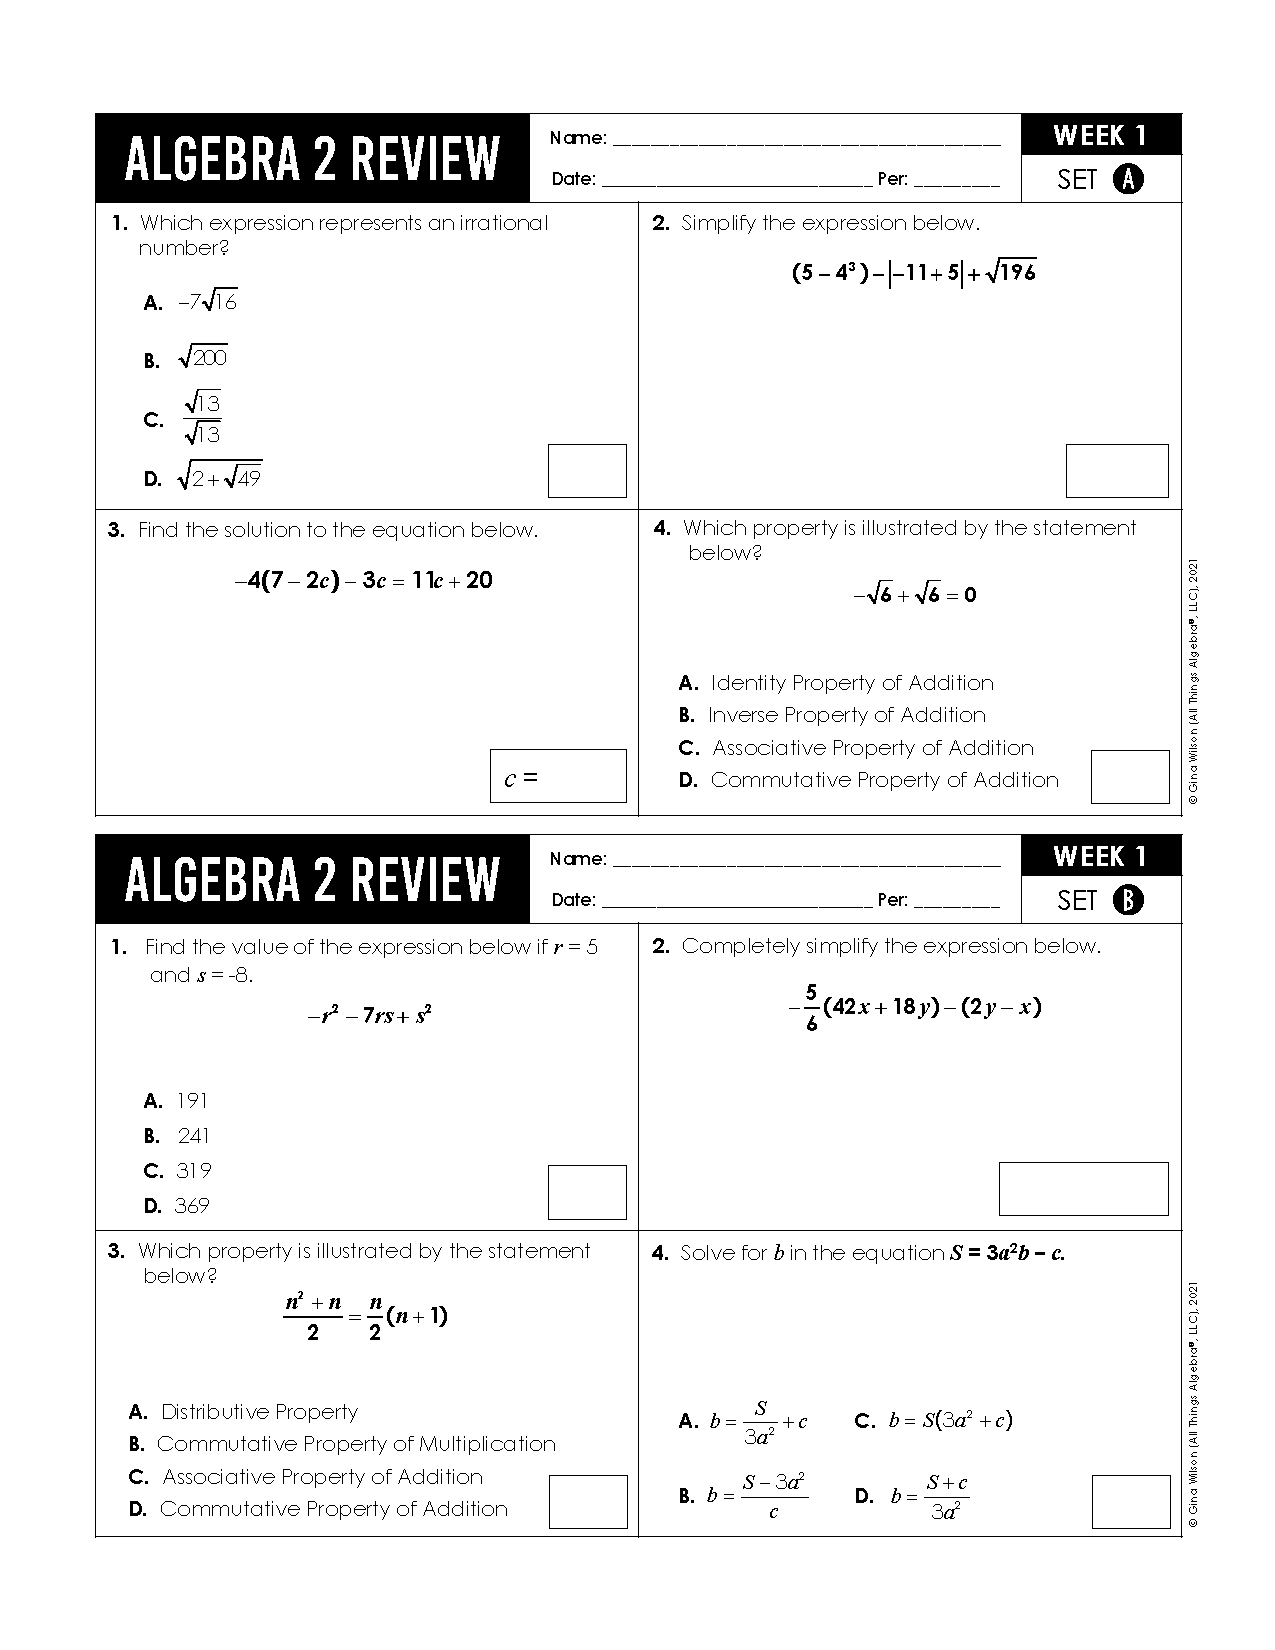
\includegraphics[width=\linewidth,page=1]{Unit1Lesson1SpiralReview1.pdf}
            \end{minipage}
        \end{tabularx}
    \end{fixedskillbox}

    \renewcommand{\arraystretch}{1.6}
    \begin{skillbox}[Hook]{sky}
        \begin{minipage}[t]{0.48\linewidth}
            \textbf{Different forms, same value} \\
            \begin{itemize}
                \item $2(x+3)$
                \item $2x+6$
                \item $x^2-9$
                \item $(x+3)(x-3)$
                \item $\sqrt{72}$
                \item $6\sqrt{2}$
            \end{itemize}
        \end{minipage}
        \hfill
        \begin{minipage}[t]{0.48\linewidth}
            \textbf{Questions}
            \begin{itemize}
                \item \textbf{Which expressions are equivalent?}
                \item \textbf{How can two expressions look different but represent the same quantity?}
                \item \textbf{How can you prove two expressions are equivalent?}
            \end{itemize}
        \end{minipage}
    \end{skillbox}

    \renewcommand{\arraystretch}{1.6}
    \begin{skillbox}[Lesson]{sky}
        \begin{multicols}{2}
            \begin{enumerate}
                \item Evaluate expressions
                \begin{itemize}
                    \item $3x^2-2x+1$ when $x=2$
                    \item \textbf{What mistakes are easy to make here?}
                \end{itemize}

                \item Simplify expressions
                \begin{itemize}
                    \item $2\left(x+5\right)-3x$
                    \item \textbf{How is the expression related to $10-x$?}
                \end{itemize}

                \item Exponent structure
                \begin{itemize}
                    \item \TallMath{\frac{x^5}{x^2}}
                    \item \textbf{What does this actually mean?}
                    \item \TallMath{\frac{x\cdot x\cdot x\cdot x\cdot x\cdot}{x\cdot x}}
                \end{itemize}
            \end{enumerate}
        \end{multicols}
    \end{skillbox}
    \begin{skillbox}[Lesson (cont.)]{sky}
        \begin{multicols}{2}
            \raggedcolumns
            \begin{enumerate}[start=4]
                \item Factoring \& Structure
                \begin{itemize}
                    \item Factor $x^2+7x+12$.
                    \item \textbf{What numbers add to $7$ and multiply to $12$?}
                    \item $x^2+7x+12=\left(x+3\right)\left(x+4\right)$
                    \item Factor $6x^2+11x+3$.
                    \item \textbf{Use slip-and-slide, multiply the constant term by the leading coefficient.}
                    \item $=x^2+11x+18$
                    \item \textbf{What numbers add to $11$ and multiply to $18$?}
                    \item $=\left( x+9 \right) \left( x+2 \right) $
                    \item $=\left( x+\frac{9}{6} \right) \left( x+\frac{2}{6} \right) $
                    \item \textbf{Simplify the fractions.}
                    \item $=\left( x+\frac{3}{2} \right) \left( x+\frac{1}{3} \right) $
                    \item \textbf{Multiply each factor by its denominator.}
                    \item $=\left( 2x+3 \right) \left( 3x+1 \right) $
                \end{itemize}
                \columnbreak
                \item Radical Simplification
                \begin{itemize}
                    \item $\sqrt{72}$
                    \item \textbf{What is the highest perfect square that is a factor of $72$}
                    \item $\sqrt{36\cdot 2}$
                    \item $6\sqrt{2}$
                    \item \textbf{a radical is simplified if no other perfect roots exist under the radical}
                \end{itemize}
            \end{enumerate}
        \end{multicols}
    \end{skillbox}

    \renewcommand{\arraystretch}{1.6}
    \begin{skillbox}[Explicit Instruction: Expression Evaluation]{sky}
        \begin{multicols}{2}
            \raggedcolumns
            \begin{enumerate}[label=\arabic*.]
                \item Identify the variables. If the expression contains $x$ or $y$,
                change the variables to $a$, $b$, $c$, etc. and set their values
                according to the specified values set forth in the problem definition.
                \item Input the expression into desmos. Double check that you have entered
                the expression correctly using the appropriate substitutions for $a$, $b$, ...
                \item Set the values of your sliders to the appropriate values for each variable.
                \item The value of your expression will be populated with the correct result, here $-10$.
            \end{enumerate}
            \columnbreak
            \textbf{Example:}
            \begin{enumerate}[label=\arabic*.]
                \item Evaluate $3x^2-2y+4z$ when $x=-2$, $y=5$, and $z=-3$.
                \item Change $x$, $y$, $z$ to $a$, $b$, $c$: $3a^2-2b+4c$.
                \item Add sliders for $a$, $b$, and $c$.
                \item Set the values accordingly: $a=-2$, $b=5$, and $c=-3$
                \item Note the value of the expression is displayed in the lower
                right corner of the first cell, here $-10$
                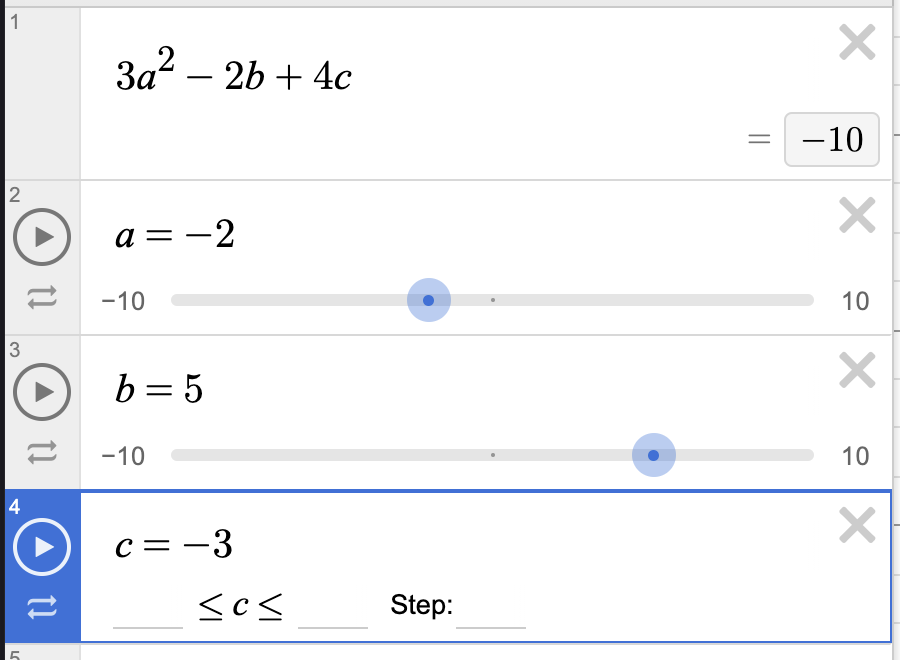
\includegraphics[width=\linewidth,page=1]{EvaluateExpressionDesmosExample}
            \end{enumerate}
        \end{multicols}
    \end{skillbox}

    \renewcommand{\arraystretch}{1.6}
    \begin{skillbox}[Explicit Instruction: Simplify/compare equivalent expressions]{sky}
        \begin{multicols}{2}
            \raggedcolumns
            \begin{enumerate}[label=\arabic*.]
                    \item Similar to above, identify the variables. If the expression contains $x$ and $y$,
                    change the variables to $a$, $b$, $c$, etc. and set their values
                    according to the specified values set forth in the problem definition. However, if there
                    is only one variable in the expression, just use $x$.
                    \item Input the expression into desmos. Double check that you have entered
                    the expression correctly using the appropriate substitutions for $a$, $b$, or $x$
                    \item Set the values of your sliders to the appropriate values for each variable if using $a$ and $b$.
                    \item If this is a multiple choice question, input the other expressions and find the one
                    that has an equivalent value to the original expression when using $a$ and $b$, or find the
                    expression's graph that perfectly lines up with the original expression.
                    \item Examples:
                    \begin{enumerate}[label=\arabic*.]
                        \item Find the simplified equivalent expression for:
                        \TallMath{\frac{x^4 \cdot x^3}{x^2}}
                        \begin{enumerate}[label=\Alph*.]
                            \item $x^5$
                            \item $\frac{x^6}{x}$
                            \item $x^9$
                            \item $x^6$
                        \end{enumerate}
                        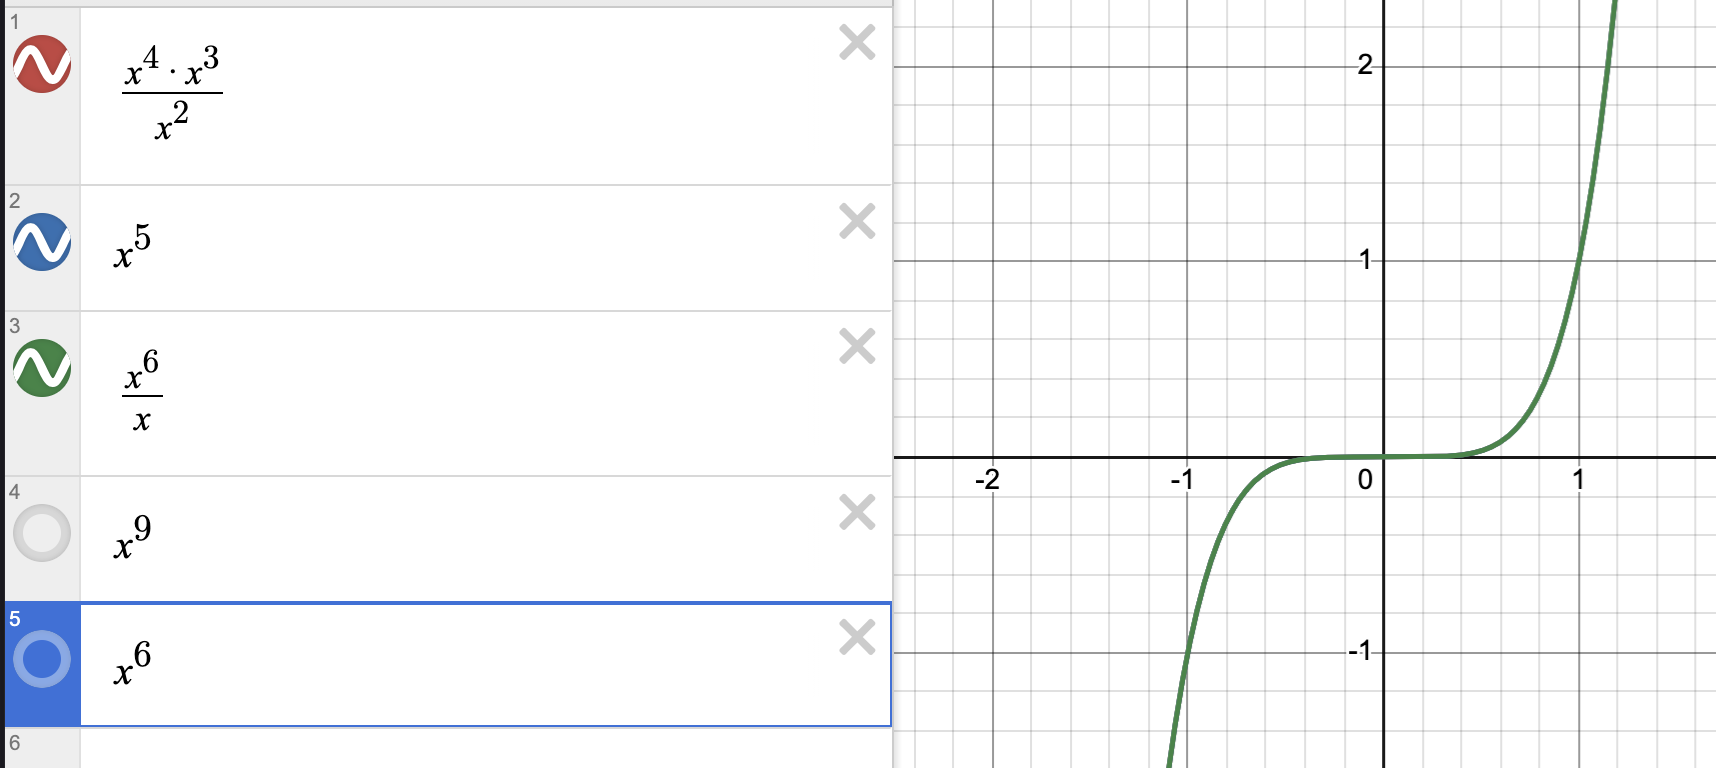
\includegraphics[width=\linewidth,page=1]{SimplifyExpressionDesmosExample}
                    \end{enumerate}
            \end{enumerate}
        \end{multicols}
    \end{skillbox}
    \begin{skillbox}[Explicit Instruction: Factor quadratics]{sky}
        \begin{multicols}{2}
            \raggedcolumns
            \begin{enumerate}[label=\arabic*.]
                    \item Most of the time, you will have a quadratic in one variable
                    that you are being asked to factor, so most of the time you will simply use $x$.
                    \item \textbf{How do you know if a quadratic is factorable?}
                    \item Input the quadratic into desmos. Double check that you have entered
                    the quadratic correctly.
                    \item Find the zeros. If the zeros of your quadratic are integers, then your factors
                    are the opposite sign of your zeros. Example, if you have zeros at 4 and -5, then
                    the factors are $\left( x-4 \right)\left( x+5 \right)$.
                    \item If the zeros are rational, this is similar to the slip-and-slide method.
                    Once you have the zeros and create the factors, then get rid of the fraction by
                    multiplying the terms of the factor by the denominator.
                    \item Examples:
                    \begin{enumerate}[label=\arabic*.]
                        \item Factor the following expression:
                        \TallMath{10x^2-13x-3}
                        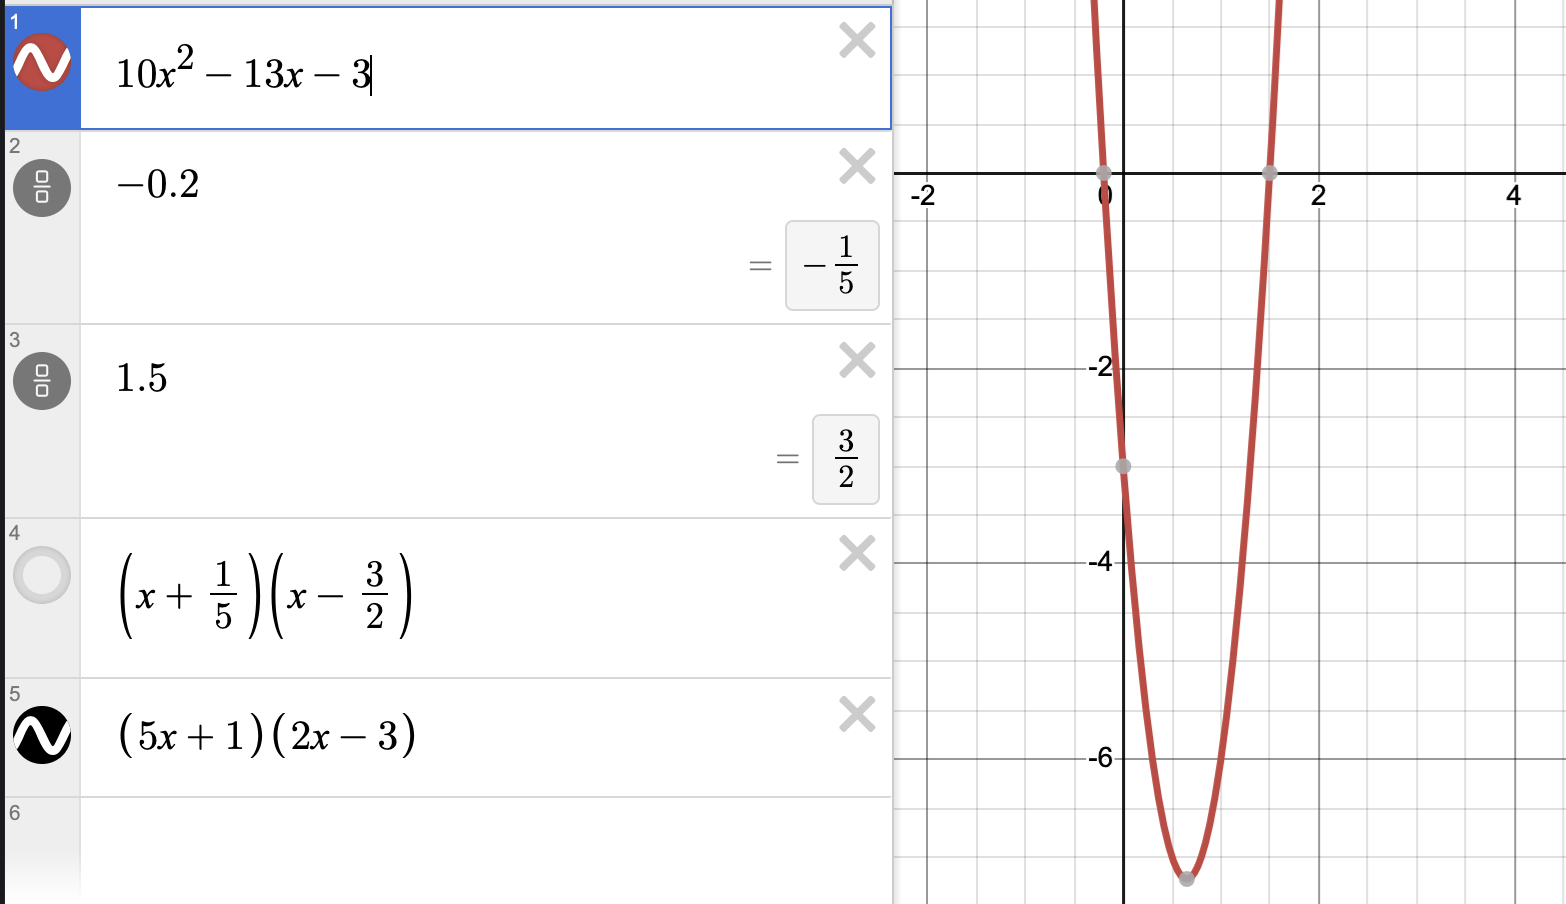
\includegraphics[width=\linewidth,page=1]{FactorQuadraticDesmosExample}
                    \end{enumerate}
            \end{enumerate}
        \end{multicols}
    \end{skillbox}
    \begin{skillbox}[Explicit Instruction: Simplify radicals]{sky}
        \begin{multicols}{2}
            \raggedcolumns
            \begin{enumerate}[label=\arabic*.]
                \item \LoremIpsum
            \end{enumerate}
        \end{multicols}
    \end{skillbox}

    \renewcommand{\arraystretch}{1.6}
    \begin{skillbox}[Active Monitoring]{redbox}
        \begin{multicols}{2}
            \raggedcolumns
            \begin{enumerate}
                \item \textbf{$3x^2 - 2y + 4z$ when $x=-2,\quad y=5,\quad z=-3$}
                \begin{itemize}
                    \item $3(-2)^2-2(5)+4(-3)$
                    \item $=3(4)-10-12$
                    \item $=12-10-12$
                    \item $=-10$
                \end{itemize}

                \item \textbf{Which expression is equivalent to and
                fully simplified form of \TallMath{\frac{x^3 \cdot x^5}{x^2}}?}
                \begin{enumerate}[label=\Alph*.]
                    \item $x^6$
                    \item $x^8$
                    \item \TallMath{\frac{x^8}{x^2}}
                    \item $x^{15}$
                \end{enumerate}
                \columnbreak
                \item \textbf{Find the fully factored form of the following two expressions:}
                \begin{itemize}
                    \item $x^2+9x+20$
                    \item $6x^2+11x+3$
                \end{itemize}
                \begin{enumerate}
                    \item \textbf{What are two numbers that add to 9 and multiply to 20?}
                    \begin{itemize}
                        \item $(x+4)(x+5)$
                    \end{itemize}
                    \item \textbf{Slip and slide when $ |a| > 1$}
                    \begin{itemize}
                        \item $6x^2+11x+3$
                        \item $=x^2+11x+18$
                        \item $=\left( x+9 \right) \left( x+2 \right) $
                        \item $=\left( x+\frac{9}{6} \right) \left( x+\frac{2}{6} \right) $
                        \item $=\left( x+\frac{3}{2} \right) \left( x+\frac{1}{3} \right) $
                        \item $=\left( 2x+3 \right) \left( 3x+1 \right) $
                    \end{itemize}
                \end{enumerate}

                \item \textbf{Which expression is equivalent to and
                fully simplified form of $ \sqrt{180} $ ?}
                \begin{enumerate}[label=\Alph*.]
                    \item $ 6\sqrt{5} $
                    \item $ 3\sqrt{20} $
                    \item $ \sqrt{36\cdot 5} $
                    \item $ 2 \sqrt{45} $
                \end{enumerate}
            \end{enumerate}
        \end{multicols}
    \end{skillbox}

    \renewcommand{\arraystretch}{1.6}
    \begin{skillbox}[Group Work \& Differentiation]{redbox}
        \textbf{\LoremIpsum}
        \par\medskip
        \hrule
        \medskip

        \begin{multicols}{3}
            \raggedcolumns
            \setlength{\columnsep}{1cm}
            \setlength{\columnseprule}{0.2pt}

            \textbf{Remediate}
            \LoremIpsum
            \columnbreak

            \textbf{Approaching Proficiency}
            \LoremIpsum
            \columnbreak

            \textbf{Extension}
            \LoremIpsum
        \end{multicols}
    \end{skillbox}

    \renewcommand{\arraystretch}{1.6}
    \begin{skillbox}[Individual Work \& Assessment]{redbox}
        \begin{minipage}[t]{0.48\linewidth}
            \LoremIpsum
        \end{minipage}
        \hfill
        \begin{minipage}[t]{0.48\linewidth}
            \LoremIpsum
        \end{minipage}
    \end{skillbox}

    \renewcommand{\arraystretch}{1.6}
    \begin{skillbox}[Reinforcement \& Extension]{goldbox}
        \begin{minipage}[t]{0.48\linewidth}
            \LoremIpsum
        \end{minipage}
        \hfill
        \begin{minipage}[t]{0.48\linewidth}
            \LoremIpsum
        \end{minipage}
    \end{skillbox}

    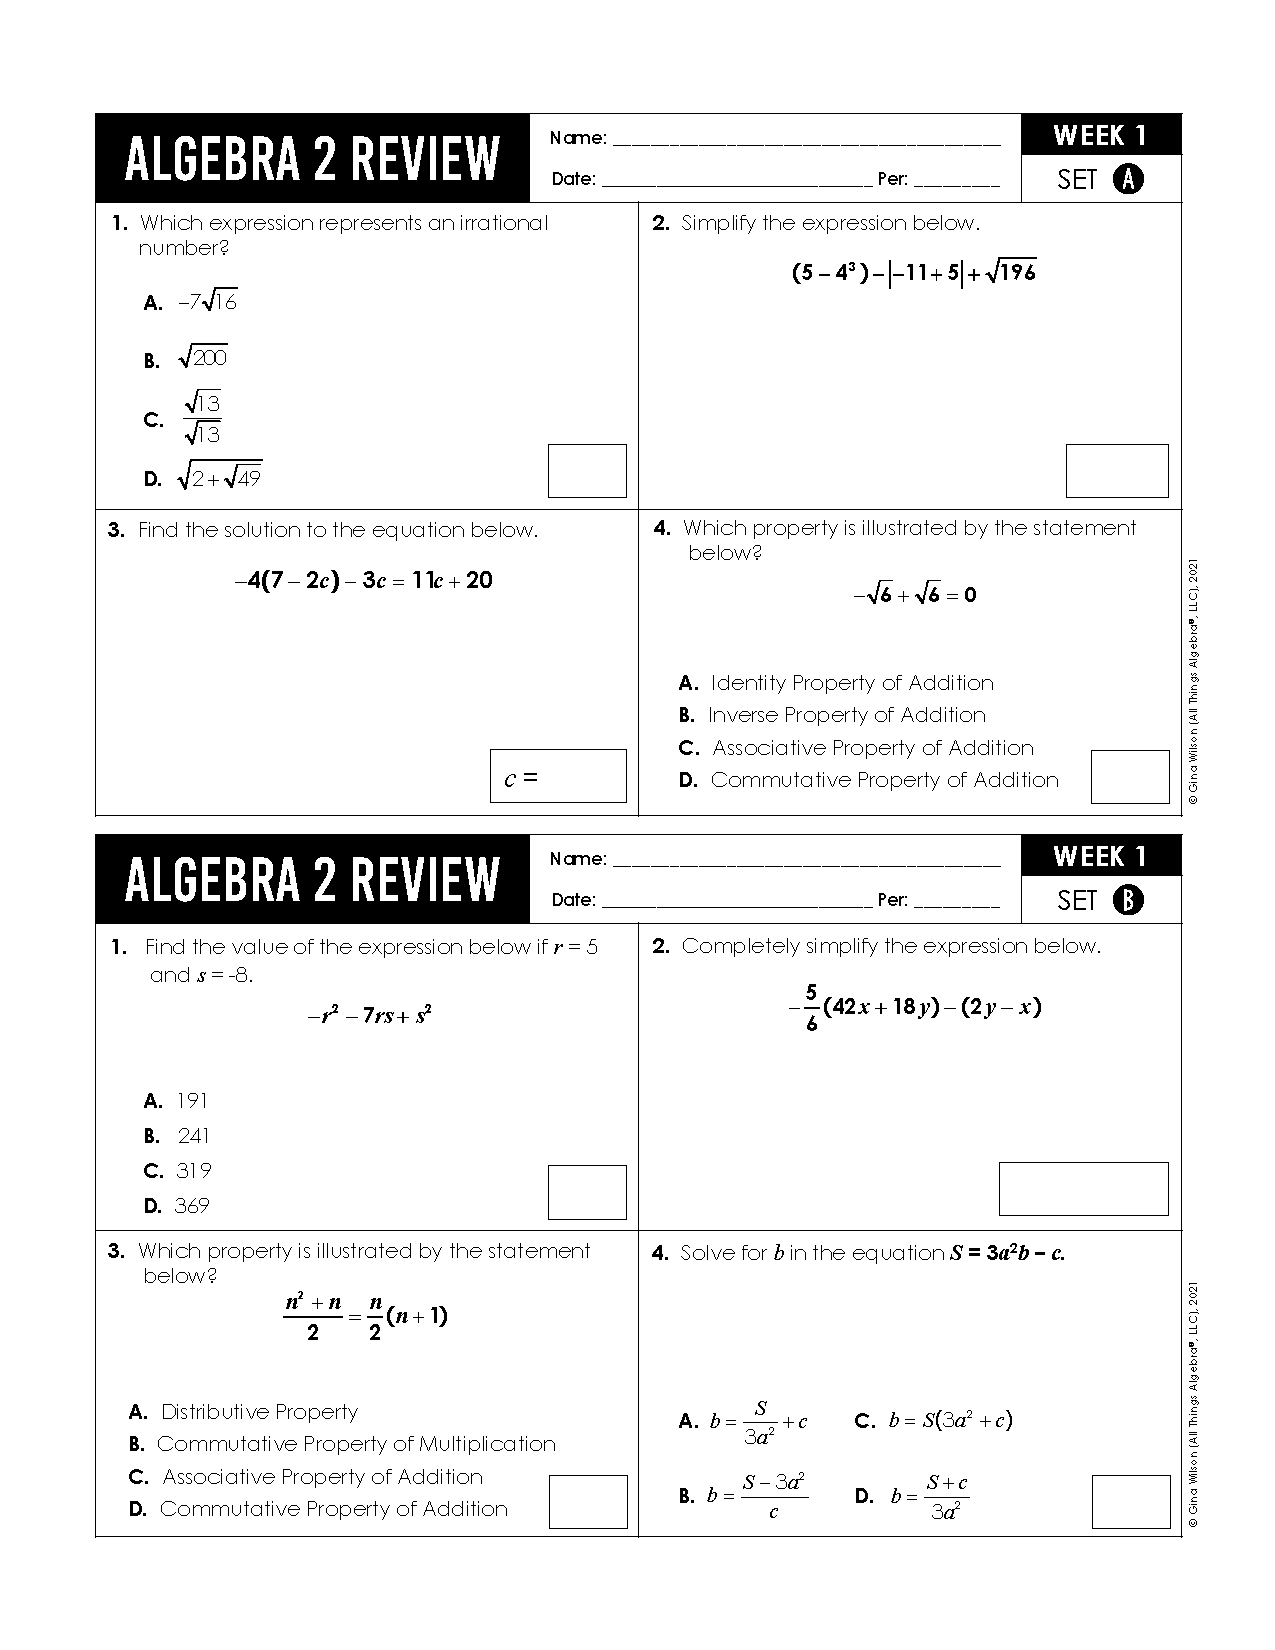
\includepdf[pages=-]{Unit1Lesson1SpiralReview1.pdf}
    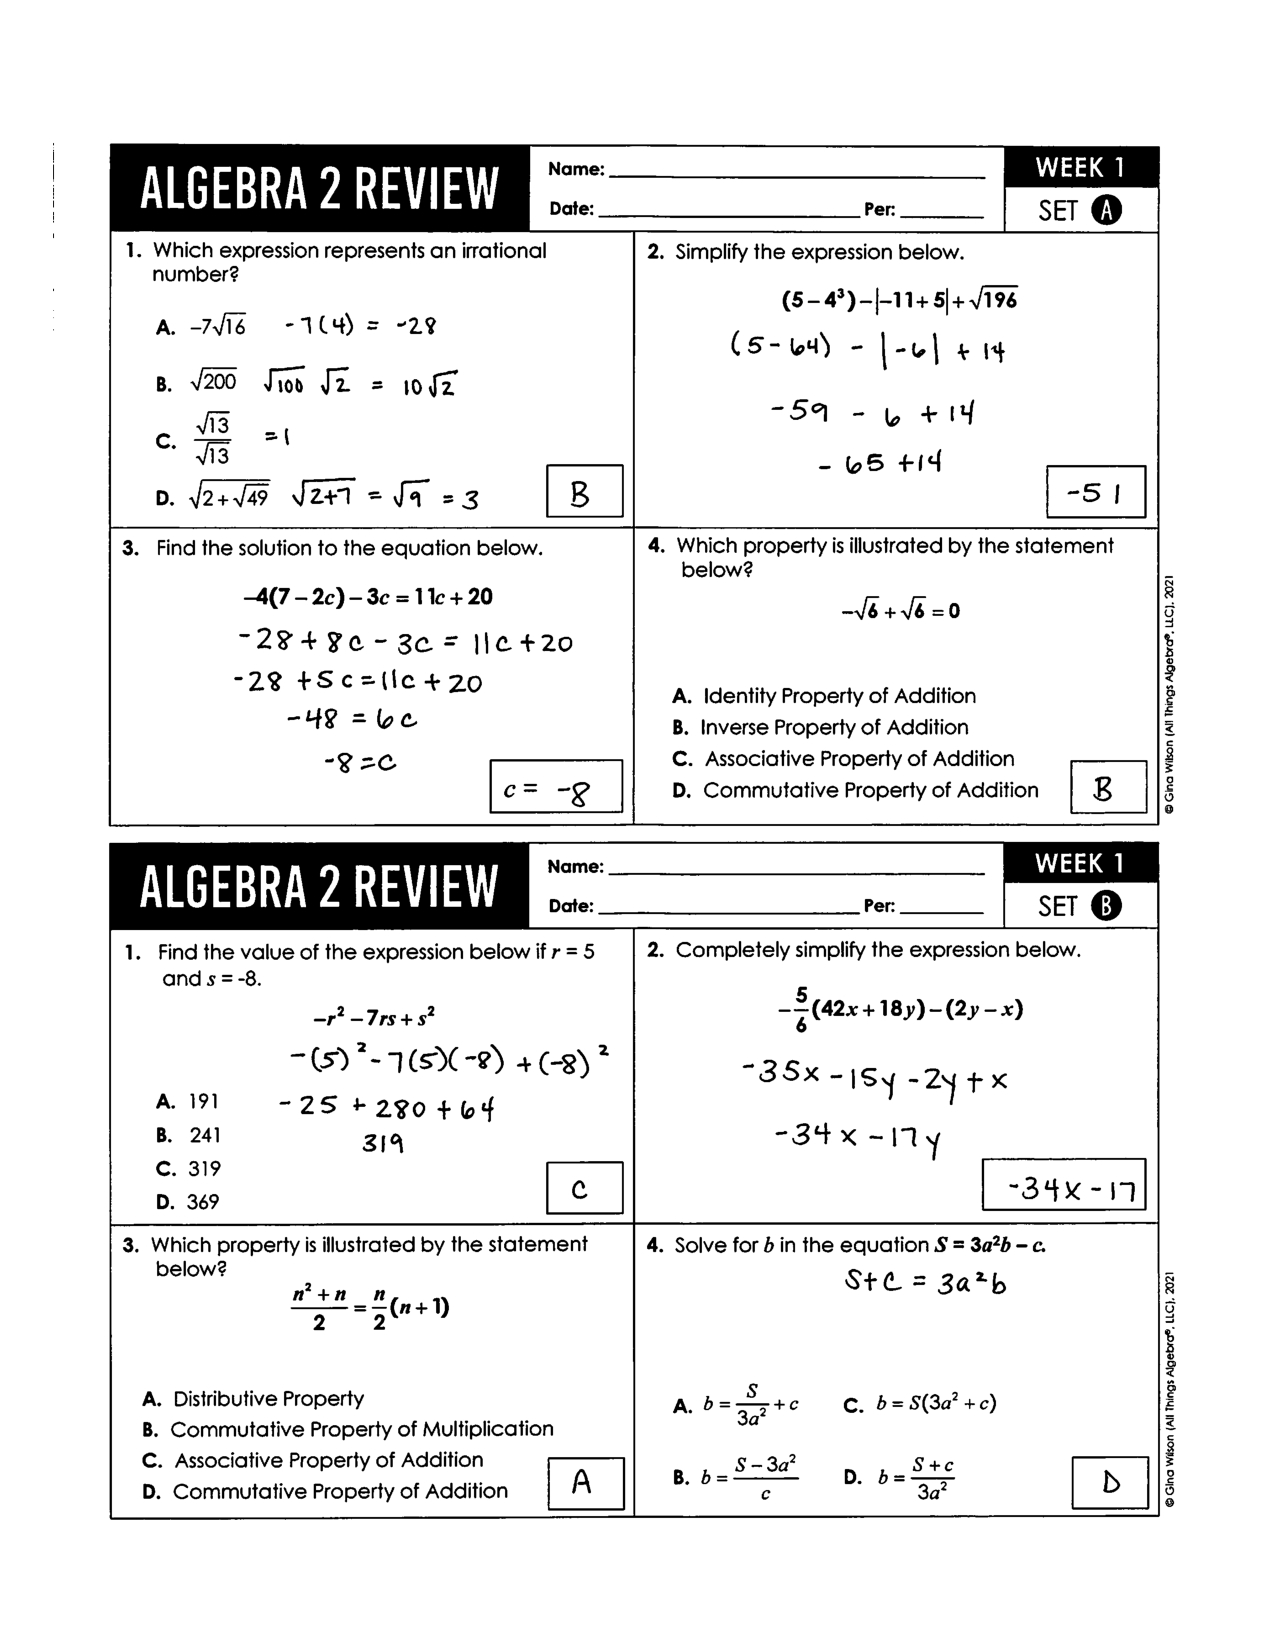
\includepdf[pages=-]{Unit1Lesson1SpiralReview1Key.pdf}
\end{document}